\chapter{Usable things}

\section{\href{https://www.sciencedirect.com/science/article/pii/S1746809421005486}{[NIYAS2021102951]}}

Epilepsy is a chronic non-communicable disease of the brain that can affect people of all ages. Around 50 million people worldwide have epilepsy, making it one of the most common neurological diseases globally. It is characterized by abnormal electrical activity causing seizures or episodes of unusual behavior, sensations, and sometimes loss of awareness [1]. It accounts for a significant proportion of the disease burden worldwide [2]. Focal Cortical Dysplasia (FCD) represents a heterogeneous group of disorders of cortical formation and is the most common cause of refractory epilepsy [3], [4]. Epilepsy is the main symptom of dysplasia, but sometimes it is also associated with mental retardation [5]. As the seizures due to FCD are difficult to control by pharmacological treatment, surgical treatment is the next viable option [5]. However, only 60–70\% of the patients enjoy a seizure-free life after the surgery [6], [7], [8]. The post-surgical seizures are due to the presence of residual dysplastic lesion caused by incomplete resection of the lesion region. Inaccurate lesion boundary estimation is the main reason behind such incomplete resection. Hence the treatment will be more effective if it is possible to identify the true extent of the lesion and perform a complete resection of the lesion [9]. However, accurate estimation of the lesion region/boundary manually through visual analysis is laborious and challenging.

\section{\href{https://ieeexplore.ieee.org/document/9198063}{[EDWIN9198063]}}

Focal Cortical Dysplasia (FCD) is a heterogeneous group of disorders due to malformations of cortical development (MCD) and is often associated with hippocampal sclerosis and cortical glioneuronal neoplasms [1]. It is considered to be the most common etiology on the cryptogenic and probable symptomatic epilepsy among adults and children [2].

Several classification systems of FCD have been proposed in the literature [3]–[6]. Palimini's [4] and Barkovich's [5] classification, is based on a two-tier system, while the ILAE classification, adopted the consensus classification system for FCD proposed by Blumcke et al. [6], which is composed of a three-tier system and shares many features with [4], [5]. It is the most widely accepted system today and differentiates the types of FCD lesions based on its location, structure, T1/T2/FLAIR signal intensities in Magnetic Resonance Images (MRI), and its adjacent occurrence with other abnormalities.

General features present in MRI images that are used to characterize FCD include cortical thickening, blurring of white-matter (WM), and gray-matter (GM) junction with the abnormal architecture of sub-cortical layer, abnormal sulcal, or gyral pattern and segmental or lobar hypoplasia [7]. FCD can be hard to detect due to its multi-focal occurrence and variable size [8]. Furthermore, the subtle characteristics of these lesions subject them to inter-observer and intra-observer variability. Consequently, automated approaches have gained popularity due to its ability to detect and quantify the extent of FCD lesions consistently.

\section{\href{https://pmc.ncbi.nlm.nih.gov/articles/PMC10933224/}{[ZHANG202403]}}

Focal cortical dysplasia (FCD) is defined as a localized malformation of cortical development caused by disturbances in neural cell proliferation, migration, and differentiation [1]. It is the most common cause of refractory epilepsy in children, accounting for more than 30\% [2]. In 2011, the International League Against Epilepsy (ILAE) classified FCD into three types according to histopathological features. Among FCD patients treated with surgical therapy, about 29–39\% were type II [3]. The final strategy for drug-resistant focal epilepsy is surgical resection. The outcome is increasingly encouraging, with 70\% of patients achieving seizure freedom [4].

Accurate pre-surgical lesion localization was the key impact factor for the outcome [5]. Three-dimension high-resolution structure MRI has become mandatory. The detailed MRI signs include cortex thickening, gray-white matter blurring, transmantle sign, and signal intensity changes in both the gray and white matter [6]. The FCD II had typical MRI features (examples shown in Fig. 1). Ordinarily, experienced neuro-radiologists can make a correct diagnosis and portray the whole lesion accurately. However, the reality is that very minimal abnormalities are reflected in subtle MRI signal alteration, which is beyond the limitations of the human eye to detect. This discrepancy is the leading cause of postoperative seizure recurrence [6].

\begin{figure}[htbp]
	\centering
	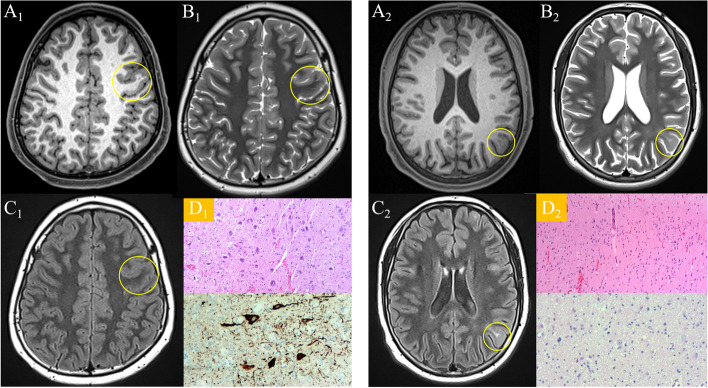
\includegraphics[width=\textwidth]{mri_12_yo.jpeg}
	\caption{Representative structure neuroimaging findings of FCD II. A1–D1 The imaging and histopathology data of a 12-year-old male patient who was diagnosed with FCD IIa. Preoperative 3D T1-MPRAGE imaging revealed localized cortical thickening and blurred gray-white matter boundary (encircled) in the left precentral gyrus. A2–D2 The imaging and histopathology data of a 15-year-old male patient who was diagnosed with FCD IIb. Preoperative FLAIR imaging demonstrated a hyperintense lesion extending into the lateral ventricle (transmantle sign, circled) in the left parietal lobe}%
\end{figure}

\section{\href{https://www.sciencedirect.com/science/article/pii/S0925231224001899}{[GANJI2024127418] better cite [AHMED2016]}}

Currently, diagnosis and analysis are still done manually, and radiologists and specialists usually spend 30 minutes for each case, and with a high probability of error, they may only find the approximate location of the lesion, and in some cases, lesions even no detectable [47]. The percentage of missing lesions in visual analysis by experts has been reported as 45–60\% [48].

\section{\href{https://hal.science/tel-02062210v2/file/these.pdf}{[alaverdyan:tel-02062210]}}

On MRI, the FCD lesions may be characterized with [Kabat and Król, 2012]
1. increased thickness of the cortical gray matter
2. blurring of the gray-white matter junction
3. increased T2 and fluid attenuated inversion recovery (FLAIR) signal intensity in the
subcortical white and gray matter
4. abnormal sulcal or gyral pattern
